\documentclass[conference]{IEEEtran}
\IEEEoverridecommandlockouts

\usepackage{cite}
\usepackage{enumitem}
\usepackage{array}
\usepackage{amsmath,amssymb,amsfonts}
\usepackage{algorithmic}
\usepackage{graphicx}
\usepackage{textcomp}
\usepackage{url}
\usepackage{listings}
\usepackage{xcolor}
\usepackage{hyperref}

\urlstyle{same}

\def\BibTeX{{\rm B\kern-.05em{\sc i\kern-.025em b}\kern-.08em
    T\kern-.1667em\lower.7ex\hbox{E}\kern-.125emX}}
    
\setlength\parindent{0pt}
\raggedbottom

\begin{document}

\title{{\huge\bf Air Traffic Flow Management: A Comprehensive Study on Operations Research in Transportation Systems}\\ {\Large\it ME 308 Project Report}}
\author{
\IEEEauthorblockN{\large Om Prabhu}
\IEEEauthorblockA{\large 19D170019}
\and
\IEEEauthorblockN{\large Vishal Srivastava}
\IEEEauthorblockA{\large 19D110025}
\and
\IEEEauthorblockN{\large Bijja Sai Kalyan}
\IEEEauthorblockA{\large 190100037}
\and
\IEEEauthorblockN{\large Balla Sarat Chandra}
\IEEEauthorblockA{\large 180100025}
}

\maketitle

\begin{abstract}
During the 120 years since the first ever flight of the Wright brothers, the air transport industry has become a major sector of the global economy. Needless to say, this growth has come with an increase in congestion and flight delays. Operations research (OR) has and continues to play a critical role in helping sustain this growth rate and make air travel more convenient.
\vspace{2mm}

In this project, we address the problem of air traffic flow management (ATFM) in response to adverse weather conditions. ATFM is the process of strategic scheduling of departures and modification of trajectories when faced with dynamically changing conditions, thereby reducing delay costs and congestion. Weather is estimated to cause nearly two-thirds of flight delays. For example, between 2004 and 2017, around 22\% of flights were either delayed or cancelled owing to adverse weather. Given the recent cyclonic developments around the Indian subcontinent, this problem is becoming increasingly relevant to Indian air traffic control systems as well.
\end{abstract}

\section{\large Introduction}
\label{sec:sec1}
\vspace{1mm}

Today, air traffic flow prediction is performed by propagating trajectories of individual flights forward in time and using them to count the number of aircraft in a region of the airspace. Examples of systems that used this approach for demand forecasting include the Future ATM Concepts Evaluation Tool (FACET), Center TRACON Automation System and the Collaborative Routing Coordination Tool. Although these systems are automated, they still require a significant amount of human intervention in irregular conditions. They are hence unreliable in the face of adversity, when split-second decisions need to be made.
\vspace{2mm}

There are two main challenges when concerned with developing ATFM algorithms. Firstly, weather conditions are highly uncertain and dynamic in nature. This poses a requirement for algorithms that can be easily updated in the event of new information without having a major impact on other aircraft routes. Secondly, the increasing amount of flight connectivity means that the same aircraft may operate multiple flights in a day resulting in delay propagation.
\vspace{2mm}

Primitive ATFM algorithms are resource-heavy since they deal with space-time trajectories of individual aircraft. In order to overcome the computational challenges of these models, many researchers have resorted to algorithms that use aggregate flows. Aggregate models simplify the design and analysis of many complex systems. Over time, Eulerian models have proved suitable for such types of feedback control systems in centralized, decentralized as well as distributed network settings (such as multi-airport networks). We discuss a similar model that is capable of processing flight data and training neural networks to calculate and display optimal flight routes.

\section{\large The Problem}
\label{sec:sec2}
\vspace{1mm}

We consider a problem with $n$ centers of the airspace and a day divided into $k$ equal time intervals. Given the time allotted for the project, we narrow the scope of the problem down to $n=3$ and $k=8$. We attempt to optimise the number of aircraft departing from \& arriving in each center as well as travelling between centers so that the total cost of ground holding and airborne delay is minimized.
\vspace{2mm}

We define a `center' as a region of the airspace with well defined, non-intersecting boundaries. A center need not be just an airport or even the airspace surrounding it - in fact, we use a broad definition wherein there can be multiple airports with one center. However, for our analysis, we consider flights departing from and arriving at only one airport within any given center and ignore all air traffic originating from the remaining airports.
\vspace{2mm}

The following image provides a better visual representation of the problem:
\begin{center}
    \centerline{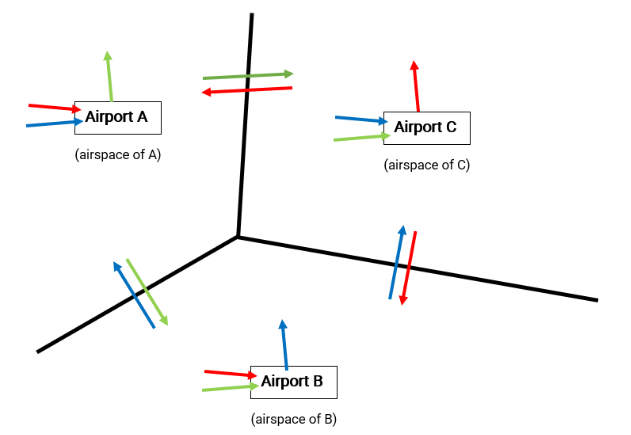
\includegraphics[width=8.5cm]{problem_description.png}}
    \textit{Fig 1: Visual representation of the problem}
\end{center}

Finally, we also list some assumptions we make to ensure the problem does not extend beyond the scope of this course:
\begin{enumerate}[label={[\arabic*]}]
    \item as mentioned earlier, we restrict $n=3$ and $k=8$
    \item all aircraft are identical in size and capacity, which makes it safe to assume that the costs associated with time delay \& ground holding is equal for all aircraft
    \item there are no connecting flights
    \item we only consider flights travelling between the 3 designated airports (eg: center A may have flights travelling from airport A to airport D - these flights are not considered)
    \item arrivals at and departures from airports occur at the time boundary between two successive time intervals
    \item transition of aircraft across airspace boundaries of centers also occur at the time boundary between two successive time intervals
    \item we do not account for stochasticity in the form of adverse weather conditions, airport crowd congestion, natural disasters, etc
\end{enumerate}

\section{\large Problem Formulation}
\label{sec:sec3}
\vspace{1mm}

We first define some basic notation for parameters and decision variables as follows:
\vspace{-0.5mm}

\begin{center}
    \bf Parameters
\end{center}
\vspace{2mm}

\begin{tabular}{@{}p{5.5em}p{0.8em}p{16.5em}@{}} 
  ArrivLim$_i(k)$ & $=$ & limit on arrivals at the airport in center $i$ during time interval $k$ \\
  $C_a,i$ & $=$ & cost of holding aircraft in the airspace of center $i$ (airborne delay cost) \\
  $C_g,i$ & $=$ & cost of holding aircraft at the airport in center $i$ (ground holding cost) \\
  Capacity$_i(k)$ & $=$ & capacity of the airport in center $i$ during time interval $k$ \\
  DeptLim$_i(k)$ & $=$ & limit on departures from the airport in center $i$ during time interval $k$ \\
  SchDept$_i(k)$ & $=$ & scheduled departures from the airport in center $i$ during time interval $k$ \\
  TrafLim$_{ij}(k)$ & $=$ & limit on traffic flow between centers $i$ and $j$ during time interval $k$ \\
  $x_i(k)$ & $=$ & total number of aircraft in center $i$ at the start of time interval $k$ \\
\end{tabular}
\vspace{-0.5mm}

\begin{center}
    \bf Decision Variables
\end{center}
\vspace{2mm}

\begin{tabular}{@{}p{5.5em}p{0.8em}p{16.5em}@{}} 
  $A_i(k)$ & $=$ & total number of arrivals at the airport in center $i$ during time interval $k$ \\
  $\beta_{ij}(k)$ & $=$ & fraction of airborne aircraft that move from center $i$ to center $j$ during time interval $k$ \\
  $D_i(k)$ & $=$ & total number of departures from the airport in center $i$ during time interval $k$ \\
\end{tabular}
\vspace{2mm}

The data for scheduled departures was obtained from a real-life daily average dataset of the airports in Mumbai, Delhi and Hyderabad respectively.
\vspace{5mm}

The following constraints were then imposed on the variables:

\begin{itemize}
    \item Balance Constraint: for $i\neq j$
$$x_i(k+1)=x_i(k)-\left(\sum\limits_{\substack{j=1\\k=1}}^{\substack{j=3\\k=7}}\beta_{ij}(k)x_i(k)+A_i(k)\right)+$$ $$\hspace{39mm}\left(\sum\limits_{\substack{j=1\\ k=1}}^{\substack{j=3\\k=7}}\beta_{ji}(k)x_j(k) + D_i(k)\right)$$
    \item Constraint on $\beta$: for every $i$ and $k$
$$\sum_{j}\beta_{ij}(k)\leqslant 1$$
    \item Departures Constraint:
$$D_i(k)=\sum_{j}\beta_{ij}(k+1)x_i(k+1)$$
    \item Arrivals Constraint:
$$\sum_{j}\beta_{ji}(k-1)x_j(k-1)\geqslant A_i(k)$$
    \item Airport Capacity Constraint:
$$A_i(k)+D_i(k)\leqslant\text{Capacity}_i(k)$$
    \item Departure Limit Constraint:
$$0\leqslant D_i(k)\leqslant \text{DeptLim}_i(k)$$
    \item Arrival Limit Constraint: 
$$0\leqslant A_i(k)\leqslant \text{ArrivLim}_i(k)$$
    \item Intercenter Flow Constraint: for $i\neq j$
$$\beta_{ij}(k)x_i(k)+\beta_{ji}(k)x_j(k)\leqslant\text{TrafLim}_{ij}(k)$$
\end{itemize}
\vspace{-1mm}

\section{\large The Cost Function}
\label{sec:sec4}
\vspace{1mm}

Recalling our objective as described in \hyperref[sec:sec2]{[Section II]}, we formulate the cost function $\mathcal{J}(\beta,A,D)$ as follows:
\vspace{-3mm}

$$\mathcal{J}:\text{ }\sum\limits_{\substack{i=1\\ k=1}}^{\substack{i=3\\k=8}}C_{g,i}(k)\left[\text{Schdept}_i(k)-D_i(k)\right]+\hspace{25mm}$$
$$\hspace{17mm}\sum\limits_{\substack{i=1\\ k=1}}^{\substack{i=3\\k=8}}C_{a,i}(k)\left[\sum_{j=1}^{j=3}\beta_{ji}(k-1)x_j(k-1)-A_i(k)\right]$$

The first summation corresponds to the ground holding costs (i.e. cost of holding aircraft that were scheduled for departure but did not actually depart), while the second summation corresponds to airborne delay costs (i.e. delay costs of flights that were scheduled to arrive in a specific time interval but did not actually arrive). We attempt to minimize this cost function, which calculated the total delay \& holding costs incurred per day.
\vspace{2mm}

\section{\large Results}
\label{sec:sec5}
\vspace{1mm}

Now that we have defined all the parameters \& decision variables, formulated all constraints and defined the cost function, we program all the parameters, variables and constraints to get an optimal value of the cost function. The optimization software used for modelling and solving this problem is AMPL and Couenne is used as the solver.
\vspace{2mm}

The detailed code and result files can be found on the Github repository linked at the end of \hyperref[sec:sec8]{[Section VIII]}. A brief summary of the model statistics is given in the table below:
\vspace{4mm}

\begin{tabular}{@{}|p{11.36em}|p{11.36em}|@{}}
  \hline
  \textbf{Parameter} & \textbf{Value} \\
  \hline
  optimal objective value (in thousand \$) & 118.41 \\
  \hline
  total constraints & 104 \\
  \hline
  total variables & 129 (48 integer) \\
  \hline
  execution time & 0.169 sec \\
  \hline
\end{tabular}
\vspace{0mm}

\section{\large Uncertainty Analysis}
\label{sec:sec6}
\vspace{1mm}

Finally, we carry out an uncertainty analysis to verify the robustness of our solutions when subjected to noise. We do this by adding Gaussian noise to our variables $x_i(k)$ and $\text{SchDept}_i(k)$. Gaussian noise is a kind of signal noise that has a probability density function equal to that of a normal distribution, which is represented by:
$$P_G(z)=\frac{1}{\sigma\sqrt{2\pi}}\exp{-\frac{(x-\mu)^2}{2\sigma^2}}$$
\vspace{0mm}

We then observe the variation in the objective function value when the variables $\beta_{ij}(k)$, $A_i(k)$ and $D_i(k)$ take their optimal values. We vary the standard deviation of Gaussian noise up to 10\%.
\vspace{2mm}

For every single value of standard deviation, we take 200 samples which correspond to 200 noise signals from its Gaussian distribution. These samples are then added to the mean values of our objective function parameters and the corresponding cost function value is calculated for each of the 200 signals.
\vspace{2mm}

We then find the expected value of our cost function through a weighted average of the individual values of the cost function and the value of the probability density function for every noise signal for a particular standard deviation.
\vspace{2mm}

As seen from the graph alongside, the maximum deviation of the cost function from its optimal value is around 7.98\%. Further, we also observe that the value of the cost function does not vary significantly from the optimal value. Thus, we conclude that the solution obtained from our model is reasonably robust for small perturbations in environmental parameters.

\begin{center}
    \centerline{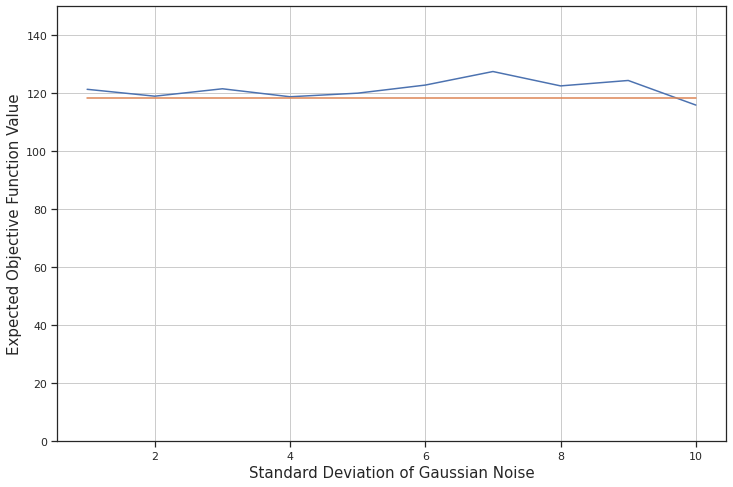
\includegraphics[width=8.5cm]{uncertainty_analysis.png}}
    \textit{Fig 2. Variation of cost function with gaussian noise}
\end{center}

\section{\large Conclusions \& Future Work}
\label{sec:sec7}
\vspace{1mm}

In this project, a linear time-varying aggregate traffic flow model has been implemented and validated against real life average data. Using the aggregate flow model, a linear program is proposed for air traffic management. Solving the optimization problem yields optimal traffic flows. Although this project discusses it in a small scale setting, the model can be adapted to fit various spatial and temporal resolutions.
\vspace{2mm}

Theoretically, this model can be extended relatively inexpensively to account for all the airports in the world. To further our work, the following improvements can be made to the existing model:

\begin{itemize}
    \item a suitable disaggregation algorithm could be implemented to extract finer instructions for every airport from the obtained results
    \item the model can be extended to even more airports/centers, which would automatically mean that we account for connecting flights as well
    \item the model can be modified to account for aircraft of different size and capacity, hence changing the ground holding \& airborne delay costs associated with each flight
    \item the complexity of the model can be increased by shrinking the time intervals to ensure more accurate predictions
    \item the results can be better visualized using an open source air traffic simulator such as openscope or bluesky
    \item the model can be extended to account for stochasticity in the form of adverse weather conditions, airport crowd congestion, natural disasters, etc - this aspect would make ATFM algorithms self-sustaining and requiring minimum human intervention
\end{itemize}
\vspace{1mm}

Note that many of these improvements are directly related to the assumptions listed in the beginning of the paper. For example, shrinking the length of time intervals gets rid of all the assumptions involving time boundaries. Overall, this makes the more more accurate and realistic.
\newpage

\section{\large References \& Links}
\label{sec:sec8}
\vspace{2mm}

\begin{enumerate}[label={[\arabic*]}]
    \item \href{https://pubsonline.informs.org/doi/epdf/10.1287/opre.1100.0899}{Dimitris Bertsimas, Guglielmo Lulli, Amedeo Odoni (2011) - An Integer Optimization Approach to Large-Scale Air Traffic Flow Management}
    \item \href{https://pubsonline.informs.org/doi/epdf/10.1287/trsc.34.3.239.12300}{Dimitris Bertsimas, Sarah Stock Patterson (2000) - The Traffic Flow Management Rerouting Problem in Air Traffic Control: A Dynamic Network Flow Approach}
    \item \href{https://pubsonline.informs.org/doi/pdf/10.1287/trsc.37.4.368.23276}{Cynthia Barnhart, Peter Belobaba, Amedeo R. Odoni (2003) - Applications of Operations Research in the Air Transport Industry}
    \item \href{https://web.mit.edu/hamsa/www/pubs/Balakrishnan_ARC2016.pdf}{Hamsa Balakrishnan (2016) - Control and Optimization Algorithms for Air Transportation Systems}
    \item \href{https://web.ics.purdue.edu/~dsun/pubs/jogcd10.pdf}{Dengfeng Sun, Banavar Sridhar, Shon Grabbe (2010) - Disaggregation Method for an Aggregate Traffic Flow Management Model}
\end{enumerate}
\vspace{2mm}

The source code (\texttt{.mod}, \texttt{.dat}, \texttt{.run}), result file, presentation file and report files (\texttt{.tex},\texttt{.pdf}) can be found on the public GitHub repository linked below:
\vspace{2mm}

\href{https://github.com/omprabhu31/ME308-Project}{\texttt{https://github.com/omprabhu31/ME308-Project}}

\end{document}
